\chapter{Fernlokalisierung mit Bluetooth}
\label{ch:phase3}
War die Infrastruktur von WLAN Access Points bisher gegeben und die Hardware somit unveränderlich, soll diese nun ausstauschbar beziehungsweise erweiterbar sein.
Dies erlaubt die Implementierung eines Bereichsortungssystems, welches nicht an die 802.11 Spezifikation gebunden ist.
Es soll eine Funkübetragungstechnik gewählt werden, die es den Tags erlaubt die in Abschnitt \ref{ch:Einleitung:sec:Anforderungen} maximal geforderten drei Jahre Akkulaufzeit zu erreichen.\\
Da mehrere Topologien für das Stationsnetzwerk denkbar sind, werden die Begriffe Basisstation und AP im Folgenden nicht mehr gleichgesetzt.
Eine Möglichkeit wäre, APs einzusetzen, die eine zweite Funkübetragungstechnik beherrschen, optional könnnte diese Fähigkeit etwa über einen USB-Port nachgerüstet werden.
Stattdessen kann die neu eingesetzte Technik auch von der bestehenden Infrastruktur getrennt und eine neue Infrastruktur aus Basisstationen aufgebaut werden.
Als Kompromiss der vorherigen Möglichkeiten können sich die neuen Basisstationen auch mittels LAN oder WLAN in die bestehende Infrastruktur einfügen. 
die Komplexität dieses Kompromisses ist geringer als bei zwei eigenständigen Netzen.

\section{nRF52832}
Der nRF52832 ist eine System-on-Chip Lösung von Nordic Semiconductor.
Er vereint eine 32-bit ARM Cortex-M4F CPU, 512kB RAM und einen 2,4GHz Transceiver, der Bluetooth 5 inklusive Low Energy und das proprietäre ANT Protokoll unterstützt \cite{nordic2017nrf}.\\
Für diese Arbeit wird ein Adafruit Feather nRF52 verwendet, der nRF52832 wird deshalb im Folgenden auf nRF52 abgekürzt.
Das Adafruit Feather nRF52 besitzt neben dem nRF52832 Spannungswandler für die 3,3 Volt Umwandlung und einen Schaltkreis für die Verwendung mit Lithium Akkus. Die verbaute CP2104 USB-to-Serial Schnittstelle erlaubt es, den Chip über USB zu programmieren.\\
Abbildung \ref{fig:nrf52layout} zeigt das Adafruit Feather nRF52.
Auch Nordic Semiconductor gibt einige typische Stromverbräuche für ihr System-on-Chip an, diese sind in Tabelle \ref{table:nrf52consumption} aufgeführt.

\begin{figure}[h]
  \centering
	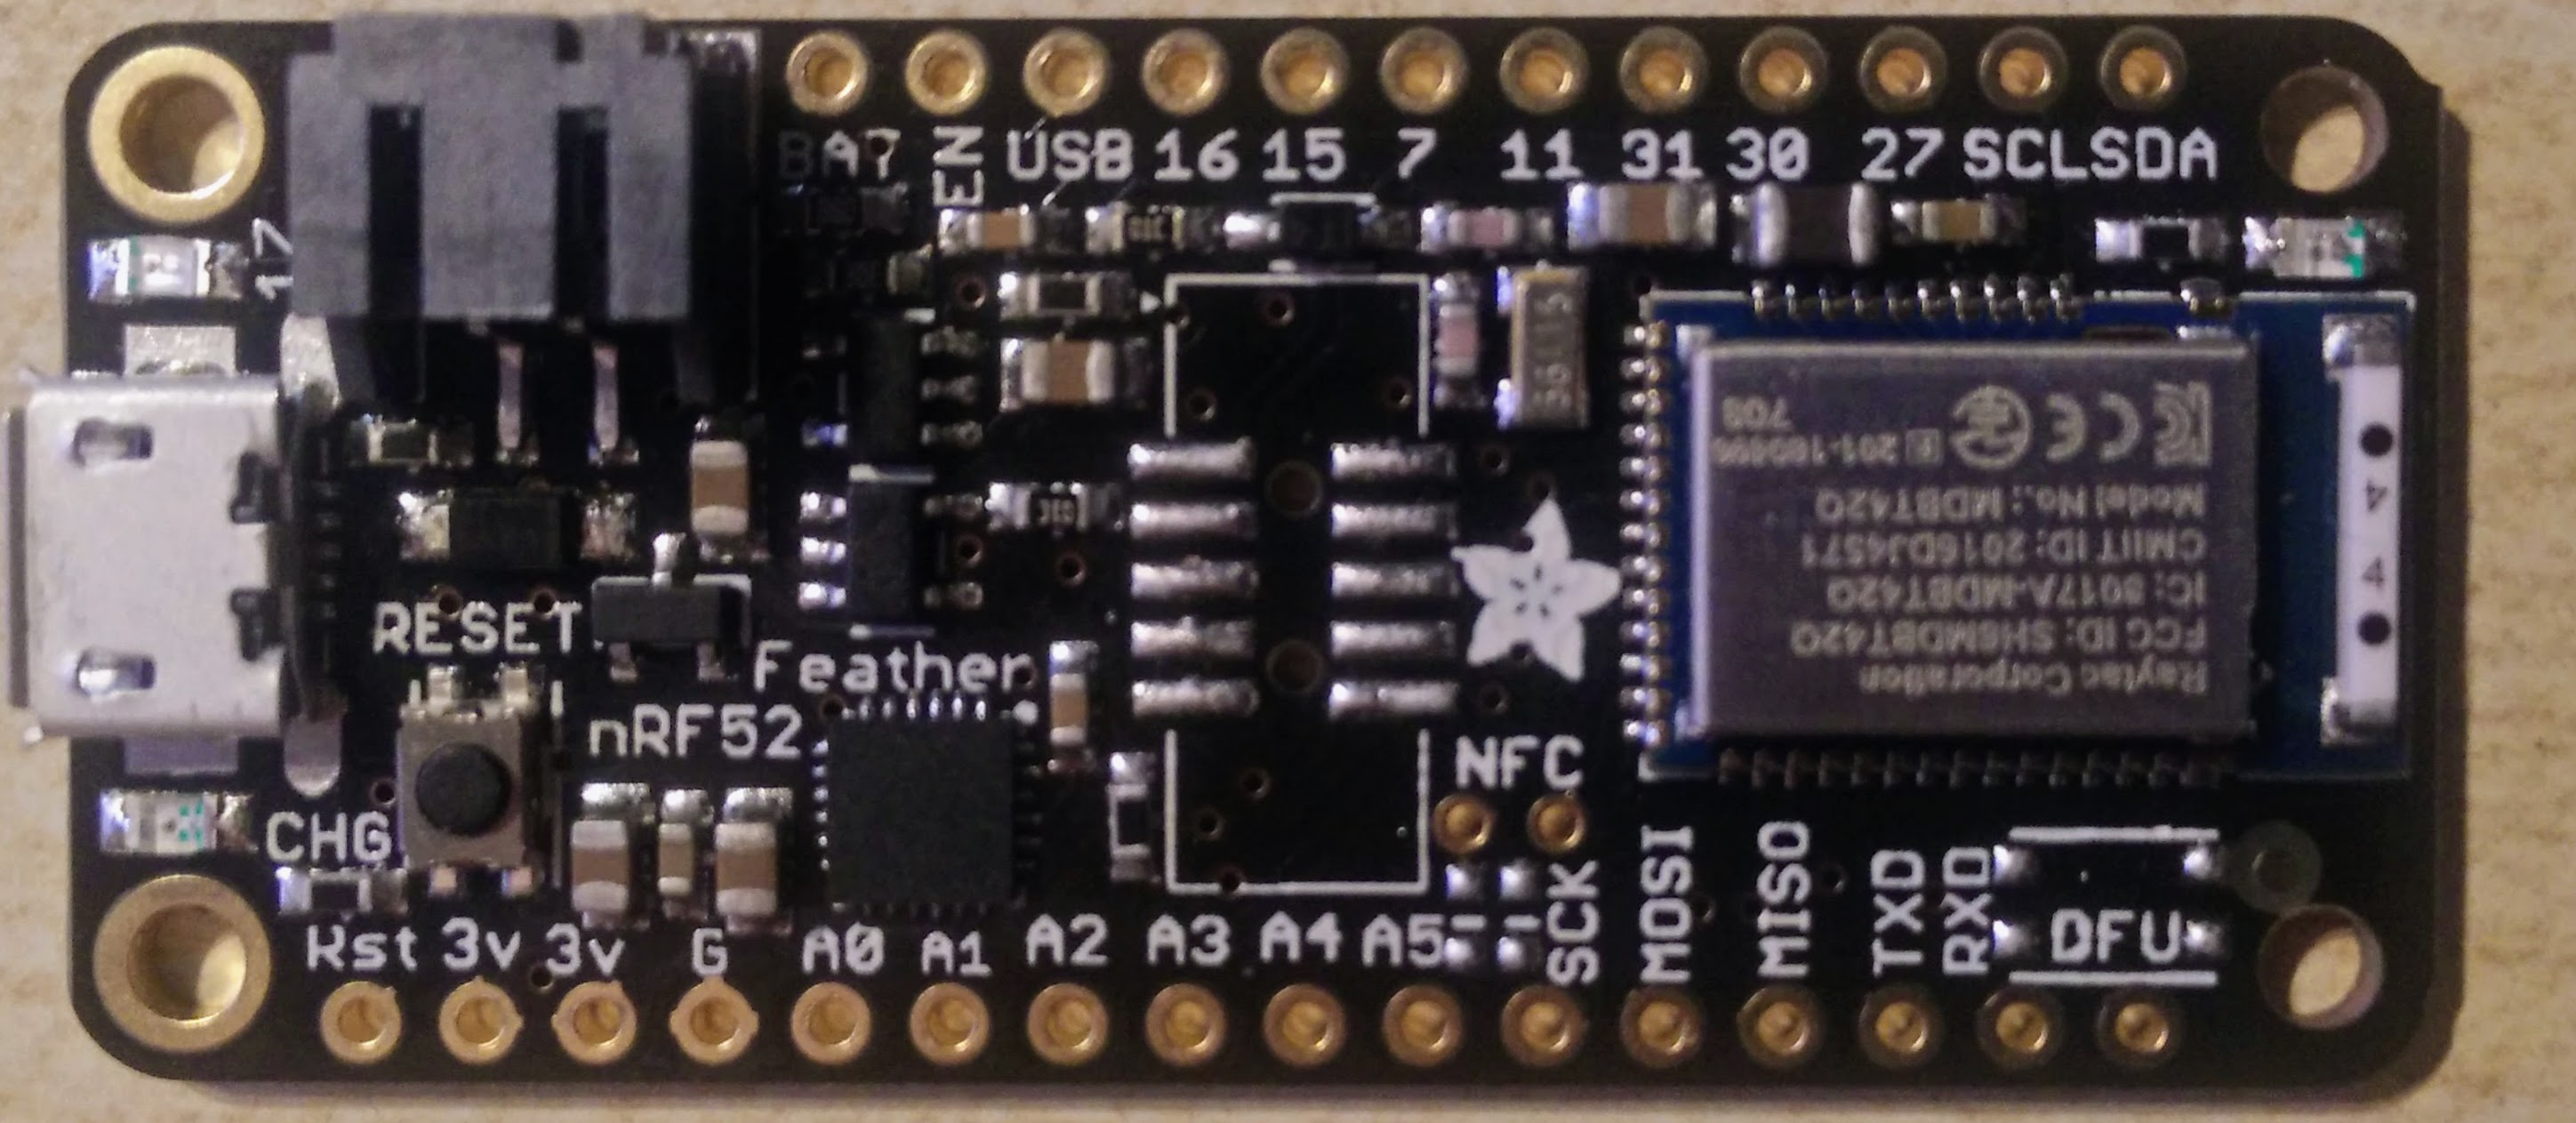
\includegraphics[width=\textwidth]{images/nrf52layout.jpg}
  \caption{Adafruit nRF52 Feather}
  \label{fig:nrf52layout}
\end{figure}

\begin{table}[h]
  \centering
  \caption{Energieverbrauch des nRF52832 in verschiedenen Zuständen, aus \cite{nordic2017nrf}}
	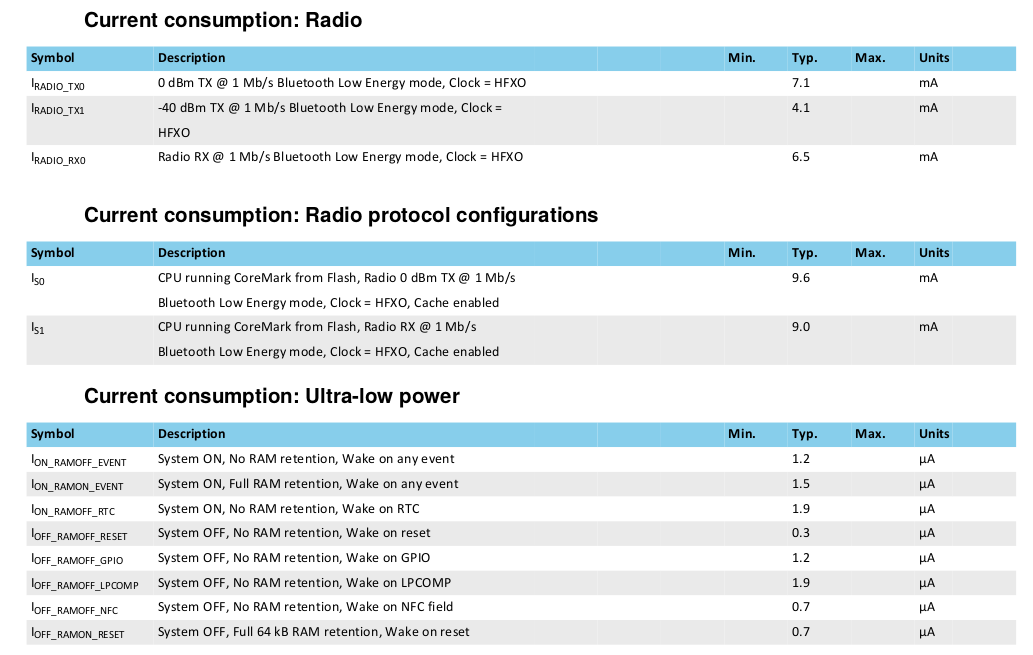
\includegraphics[width=\textwidth]{images/nrf52consumption.png}
  \label{table:nrf52consumption}
\end{table}


\subsection{Arduino Bluefruit nRF52 API}
Der nRF52 kann ebenfalls mit der Arduino IDE programmiert werden.\\
Dazu muss dieser zunächst das Board Support Package hinzugefügt werden \cite{townsend2017nrf}.
In den Einstellungen wird unter \textit{Additional Boards Manager URLs} die URL \url{https://www.adafruit.com/package_adafruit_index.json} hinzugefügt.
Nach einem Neustart der Arduino IDE kann im \textit{Boards Manager} das Paket Adafruit nRF52 installiert werden.
Um das Board programmieren zu können wird zusätzlich das \textit{nrfutil} benötigt.
Dieses liegt nach der Installation der Boards in \\\texttt{/.arduino15/packages/adafruit/hardware/nrf52/0.6.0/tools/nrfutil-0.5.2} und muss mit \texttt{sudo pip install -r requirements.txt} und \texttt{sudo python setup.py install} installiert werden.
Nachdem das Board in der IDE ausgewählt und über USB mit dem Computer verbunden wurde, kann nun eigener Code oder eines der Beispiele aus \textit{Examples for Adafruit Bluefruit nRF52 Feather} mit STRG+U auf den nRF52 geladen werden.\\
Es wird die Bluefruit nRF52 API Version 0.6.0 verwendet.

\section{BLE Advertising Implementierung}
\label{ch:phase3:sec:advertising}
Die Bluetooth Low Energy Implementierung ist an die Arbeit von Jianyong et al. angelehnt.
Es wird immer nach Ablauf des Sendeintervalls ein Advertising Paket gesendet.\\
In der Praxis wird dazu das Advertising Interval entsprechend gesetzt, dabei handelt es sich um einen in Bluetooth 4.0 spezifizierten Parameter für die Häufigkeit des Advertisings.
Da die Bluefruit nRF52 API keine Funktion zur Änderung dieses Wertes zur Verfügung stellt muss er direkt geändert werden.
Die entsprechende BLEAdvertising Klasse ist in \\\texttt{\~/.arduino15/packages/adafruit/hardware/nrf52/0.6.0/libraries/}\\\texttt{Bluefruit52Lib/src} zu finden. \\
In \texttt{BLEAdvertising.cpp} ist \texttt{GAP\_ADV\_INTERVAL\_MS} auf 20 Millisekunden gesetzt, dieser Wert sollte erhöht werden, um den Energieverbrauch zu senken.
Beim nRF52 handelt es sich um ein Klasse 2 Bluetooth Gerät mit einer maximalen Sendeleistung bis 4 dBm.
Es wird daher eine Reichweite von 20 Metern angenommen und das Sendeintervall etsprechend der maximalen Bewegungsgeschwindigkeit von 30 km/h auf eine Sekunde gesetzt. 
In dieser Zeit kann sich ein Mitarbeiter maximal 9 Meter bewegen, es werden also bei der Durchquerung des Einflussbereichs mindestens drei Advertising Pakete von der mobilen Einheit versendet.\\
Es sollte erneut eine Voruntersuchung des Verbrauchs mit dem Muker TM103 USB-Power-Meter vorgenommen werden.
Diser ist aber nicht in der Lage den Stromverbrauch des nRF52 zu messen..
Die Sendeabschnitte sind zu kurz um einen messbaren Stromverbrauch zu erzeugen.\\
Deshalb wird zunächst Abbildung \ref{table:nrf52consumption} für eine theoretische Betrachtung des Verbrauchs herangezogen werden. 

\subsection{Theoretische Energieverbrauchsabschätzung}
Für die Zeit in der nicht gesendet wird, wird der Zustand $I_{ON\_RAMOFF\_RTC}$ angenommen, da dieser den höchsten Verbrauch aufweist.
Für die Sendezeit wird $I_{RADIO\_TX0}$ angenommen, für ein Advertising Paket, welches zusätzlich den Gerätenamen "{}TestTag"{} versendet, werden 24 Bytes (192 Bit) gesendet.
Um die Kollisionsvermeidung einzufügen werden vorher 2000 Bit im Zustand $I_{RADIO\_RX0}$ empfangen, der die restliche Zeit wird in $I_{ON\_RAMOFF\_RTC}$ verbracht. 
Es müssen ebenfalls die weiteren Komponenten auf dem Feather bedacht werden. 
Adafruit gibt für den Spannungswandler einen Verbrauch von 55 Mikroamper und für den Lithium-Polymer-Ladeschaltkreis einen Verbrauch von bis zu 100 Mikroamper an \cite{fried2016lora}. 
Der Verbrauch des anderen Komponenten des Feather wird daher konservativ auf 155 Mikroamper geschätzt.\\[1cm]

$y = (1s-\frac{Bits\_gesendet}{1000000 b/s} - \frac{Bits\_empfangen}{1000000 b/s}) * (I_{ON\_RAMOFF\_RTC} + 155 {\mu}A) + \frac{Bits\_gesendet}{1000000 b/s} * I_{RADIO\_RX0} + \frac{Bits\_empfangen}{1000000 b/s} * I_{RADIO\_RX0}$\\[0.5cm]
$y = (1s - 0,000192s - 0,002s) * 0,1569mA + 0,000192 * 7,1mA + 0,002 * 6,5mA$\\[0.5cm]
$y \approx 0,156556mA + 0,001363mA + 0,013mA = 0,170919mA$ \\[1cm]

Eine Untersuchung des tatsächlichen Verbrauchs ist in Abschnitt \ref{ch:phase3:sec:powerble} zu finden.



\section{RFM95}
\label{ch:hardwarechanges:sec:rfm95}
Bei dem RFM95 handelt es sich um ein LoRa (Long Range) fähiges Radio-Modul für den Frequenzbereich 868/915MHz \cite{hope2006rfm}. 
915MHz sind jedoch nur in Amerika lizenzfrei, in Deutschland muss das Radio mit 868MHz betrieben werden.\\
Für die Entwicklung wird das Modul auf einem Adafruit Feather M0 RFM95 LoRa Radio verwendet.
Dieses verwendet zusätzlich einen M0 Mikrocontroller zur Steuerung, einen Lithium-Akku-Ladeschaltkreis und einen Spannungswandler zur einfachen Programmierung des Radios über USB.
Zusätzlich ist eine Antenne notwendig, die verwendete Antenne kann dabei einen große Unterschiede in der Reichweite verursachen, deshalb sollte eine Antenne für 868MHz verwendet werden.
Da jedoch eine feste Antenne die mobile Einheit unhandlich machen würde, wird für diese eine Kabelantenne verwendet, diese hat die Länge einer halben Wellenlänge (17,3cm).\\
Abbildung \ref{fig:lorafeather} zeigt zwei Feather M0 RFM95 LoRa Radio. 
Das RFM95 mit Kabelantenne dient als mobile Einheit und das RFM95 mit fester Antenne dient als Basisstation.

\begin{figure}[h]
  \centering
	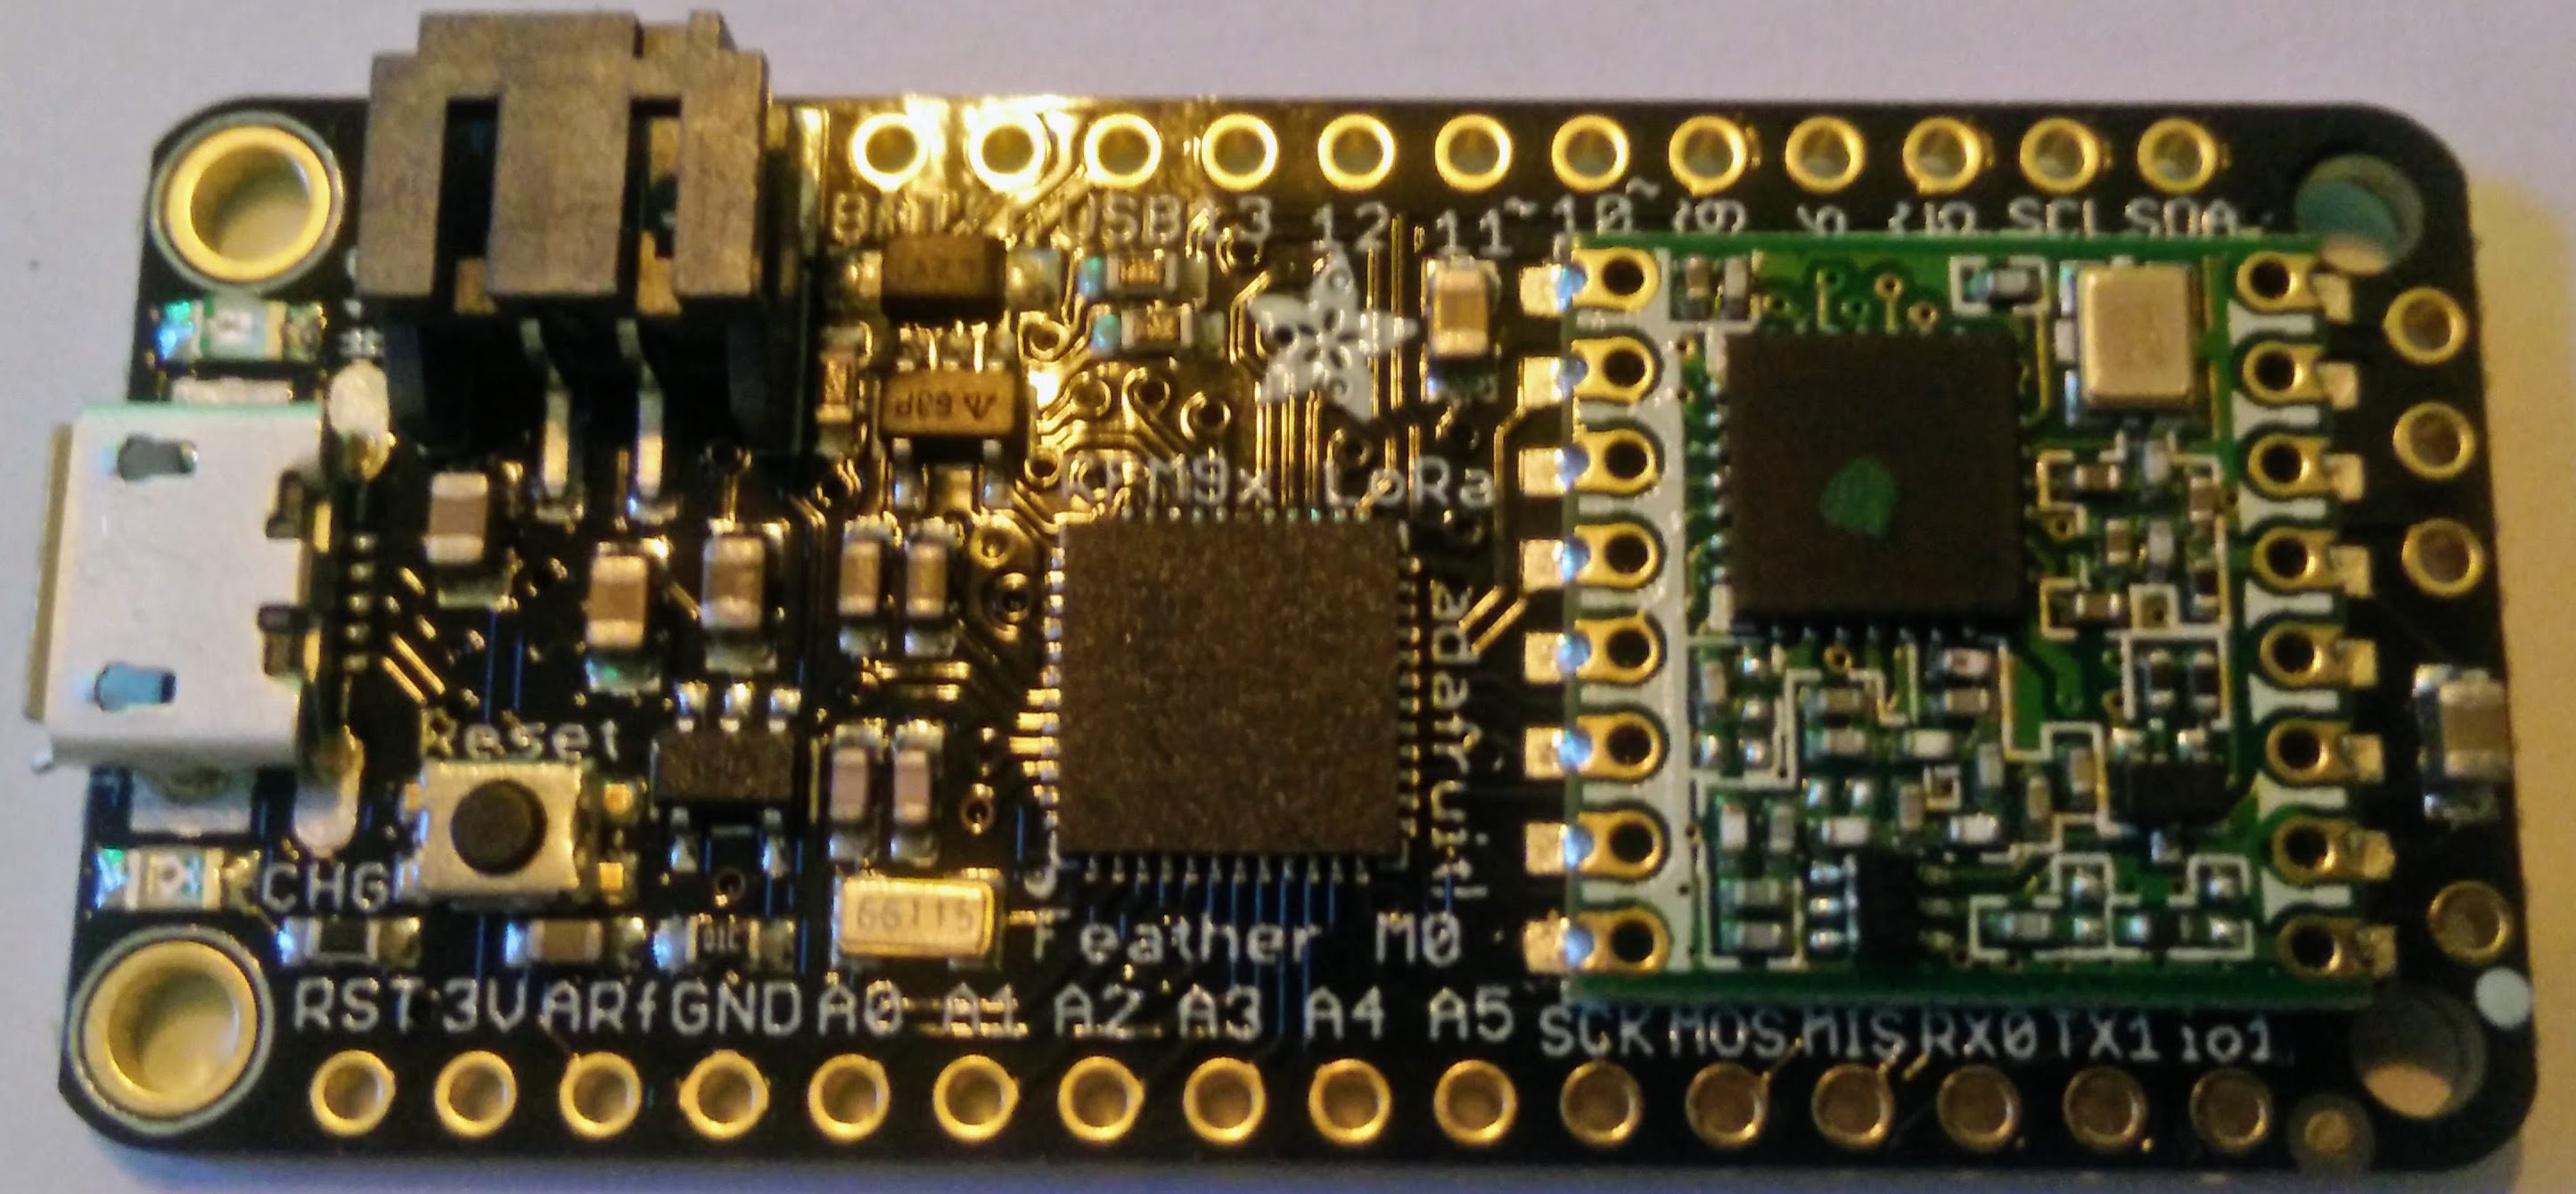
\includegraphics[width=\textwidth]{images/lorafeather.jpg}
  \caption{Adafruit LoRa Feather mit RFM95}
  \label{fig:lorafeather}
\end{figure}

\subsection{RadioHead RFM9x für Arduino}
Der M0 Mikrocontroller ist Arduino kompatibel, wird zusätzlich die RadioHead RFM9x Bibliothek verwendet, kann er über ein SPI-Interface das Radio steuern.
Dazu muss zunächst in den Optionen der Arduino IDE unter \textit{Additional Boards Manager URLs} die URL \url{https://adafruit.github.io/arduino-board-index/package_adafruit_index.json} hinzugefügt werden \cite{treece2016lora}.
Nach einem Neustart der IDE können im \textit{Board Manager} die \texttt{Arduino SAMD Boards} installiert werden. 
Der M0 kann nun programmiert werden, um das RFM95 verwenden zu können muss die RadioHead RFM9x Bibliothek von \url{https://cdn-learn.adafruit.com/assets/assets/000/035/106/original/RadioHead-1.62.zip} heruntergeladen und nach \\\texttt{/Arduino/libraries/} entpackt werden.

\section{LoRa Implementierung}
Die Implementierung für die Lokalisierung mit LoRa ist sehr simpel.
Die mobile Einheit versendet regelmäßig ein Paket, welches einen Identifikator für die mobile Einheit enthält.
Das Sendeintervall beträgt entsprechend der hohen erwarteten Reichweite 10 Sekunden.\\
Die Basisstation empfängt durchgehend und bestimmt den RSSI für eingehende Pakete.
Anschließend leitet sie den Identifikator der mobilen Einheit zusammen mit dem RSSI und einer Kennung für die Basisstation an den Ortungsserver weiter.\\
Auf der mobilen Einheit müssen lediglich die Sendefrequenz, die Sendeleistung und der Identifikator gesetzt werden, dann kann immer nach Ablauf des Sendeintervalls gesendet werden.
Die Basisstation muss dabei auf der selben Frequenz aktiv sein und empfangen.

\subsection{Theoretische Energieverbrauchsabschätzung}
Für die Berechnung des theroretischen Verbrauchs der mobilen Einheit werden die Datenblätter des M0 Mikrocontrollers und des RFM95 Radios herangezogen. 
Die dort gelisteten Verbräuche sind in Tabelle \ref{table:m0power} und Tabelle \ref{table:lorapower} zu finden.

\begin{table}[h]
  \centering
  \caption{Stromverbrauch des M0 Mikrocontrollers, aus \cite{nxp2016m0}}
	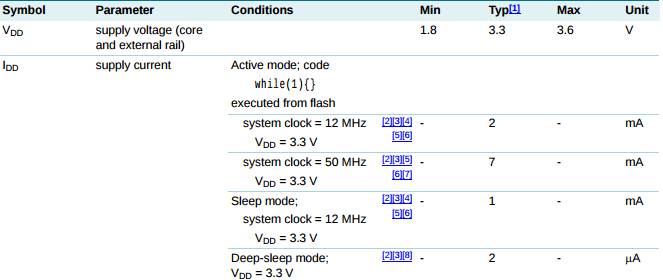
\includegraphics[width=\textwidth]{images/m0power.png}
  \label{table:m0power}
\end{table}

\begin{table}[h]
  \centering
  \caption{Stromverbrauch des RFM95, aus \cite{hope2006rfm}}
	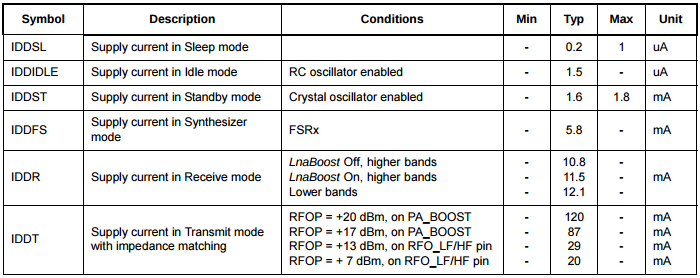
\includegraphics[width=\textwidth]{images/lorapower.png}
  \label{table:lorapower}
\end{table}

Da das Adadfruit Feather M0 RFM95 Lora Radio ansonsten baugleich zum Adafruit Feather nRF52 ist werden die 155 Mikroamper für die sonstigen Komponenten übernommen.\\
Die Sendeleistung des RFM95 Radio ist zwischen 5dBm und 23dBm einstellbar. 
Das Datenblatt listet jedoch nur Verbräuche zwischen 7dBm und 20dBm Sendeleistung, der Verbrauch wird für diese beiden Sendeleistungen berechnet.
Für die Nachricht "{}TagTest"{} werden 20 Bytes (160 Bits) versendet, es wird angenommen, dass zuvor 500 Bits für die Kollisionskontrolle belauscht werden.\\[1cm]

$y = \frac{1}{10} * [(10 - \frac{Bits\_gesendet}{21875 b/s} - \frac{Bits\_empfangen}{21875 b/s}) * (M0\_Deep\_sleep\_mode + RMF95\_IDDIDLE + 155 {\mu}A) + \frac{Bits\_gesendet}{21875 b/s} * RFM95\_XdBm + \frac{Bits\_empfangen}{21875 b/s} * RFM95\_IDDR]$\\[0.5cm]
$y_{20dBm} = \frac{1}{10} * [(10s - 0,0073s - 0,0229s) * 0,1585mA + 0,0073s * 120mA + 0,0229s * 12,1mA]$\\[0.5cm]
$y_{20dBm} \approx \frac{1}{10} * (1,58mA + 0,876mA + 0,2771mA) = 0,2683mA$\\[1cm]

$y_{7dBm} = \frac{1}{10} * [(10s - 0,0073s - 0,0229s) * 0,1585mA + 0,0073s * 20mA + 0,0229s * 12,1mA]$\\[0.5cm]
$y_{7dBm} \approx \frac{1}{10} * (1,58mA + 0,146mA + 0,2771mA) = 0,1953mA$\\[1cm]

Eine Untersuchung des tatsächlichen Verbrauchs ist in Abschnitt \ref{ch:phase3:sec:powerlora} zu finden.

\section{Untersuchung des Energieverbrauchs}
Der Energieverbrauch soll mit dem INA219 genauer bestimmt werden, der INA219 und die verwendete Methodik werden in Abschnitt \ref{ch:phase1:sec:energie} beschrieben.

\subsection{Bluetooth Low Energy Advertising}
\label{ch:phase3:sec:powerble}
Abbildung \ref{fig:blue} zeigt den Lastverlauf für den Start einer mobilen Einheit mit Bluetooth Low Energy Advertising.\\
Zu Beginn ist eine Startphase zu erkennen, ab 2 Sekunden nach Start des Experiments ist dann das regelmäßige Muster aus Verbrauch im Ruhezustand und kurzen Verbrauchsspitzen beim Senden zu erkennen.
Die Kürze des Sendevorgangs bedingt die starke Schwankung bei den Lastspitzen, die Samplingrate von 333Hz reicht hier offenbar nicht aus um dem Sendevorgang vollständig zu erfassen.\\

\begin{figure}[h!]
  \centering
	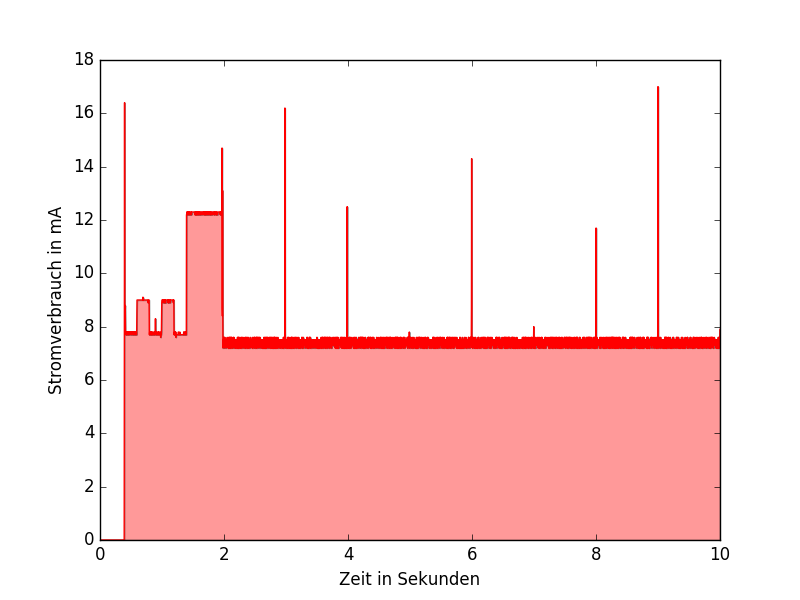
\includegraphics[width=\textwidth]{plots/blue.png}
  \caption{Lastkurve einer Implementierung von Bluetooth Low Energy Advertising.}
  \label{fig:blue}
\end{figure}

Hauptverbrauch liegt jedoch in den 7,2 bis 7,6 Milliamper im Ruhezustand, leider ist in diesem Fall kein einzelnes Modul vorhanden, es kann nur auf dem nRF52 Feather gemessen werden.
Da jedoch die selben Komponenten wie beim ESP8266 Feather zum Einsatz kommen, kann angenommen werden, dass auch der Ruheverbrauch vergleichbar ist, dieser liegt zwischen 7 und 7,1 Milliamper.
Tabelle \ref{table:blueina} zeigt deshalb neben dem gemessenen Verbrauch einen projezierten Verbrauch, bei dem ein Ruheverbrauch von 7,05 Milliamper subtrahiert wurde.

\begin{table}[h!]
	\centering
	\caption{Energieverbrauch mobiler Einheiten mit Bluetooth Low Energy Advertising}
	\label{table:blueina}
	\begin{tabular}{p{3.5cm}|p{5cm}|p{2.5cm}|p{2.5cm}}
		Hardware & Programm & $\varnothing$ Verbrauch in mA & Laufzeit in Stunden\\
		\hline
		nRF52 Feather & Bluetooth Low Energy Advertising & 7,37 & 190\\
		nRF52 (projeziert) & Bluetooth Low Energy Advertising & 0,32 & 4375\\
	\end{tabular}
\end{table}

\subsection{Lokaliserung mit LoRa}
\label{ch:phase3:sec:powerlora}
Der Stromverbrauch der Implementierung mit LoRa wurde mit 5dBm und 23dBm Sendeleistung überprüft
Abbildung \ref{fig:lora23} zeigt den Lastverlauf für den Start einer mobilen Einheit mit LoRA bei 23dBm.\\
Nach einer circa drei sekündigen Startphase wechselt der LoRa Feather in den regulären Betrieb, er sollte dann immer nach zehn Sekunden Ruhezustand senden.
Dieser jedoch vom Zeitgeber nicht ganz eingehalten, die mobile Einheit befindet sich zwischen den Sendevorgängen circa elf Sekunden im Ruhezustand, dies sollte bei der Implementierung beachtet werden.
Im Ruhezustand liegt der Verbrauch des LoRa Feather bei 2,5 bis 2,7 Milliamper, beim Senden unterscheiden sich die Vebräuche je nach Sendeleistung deutlich.\\

\begin{figure}[h!]
  \centering
	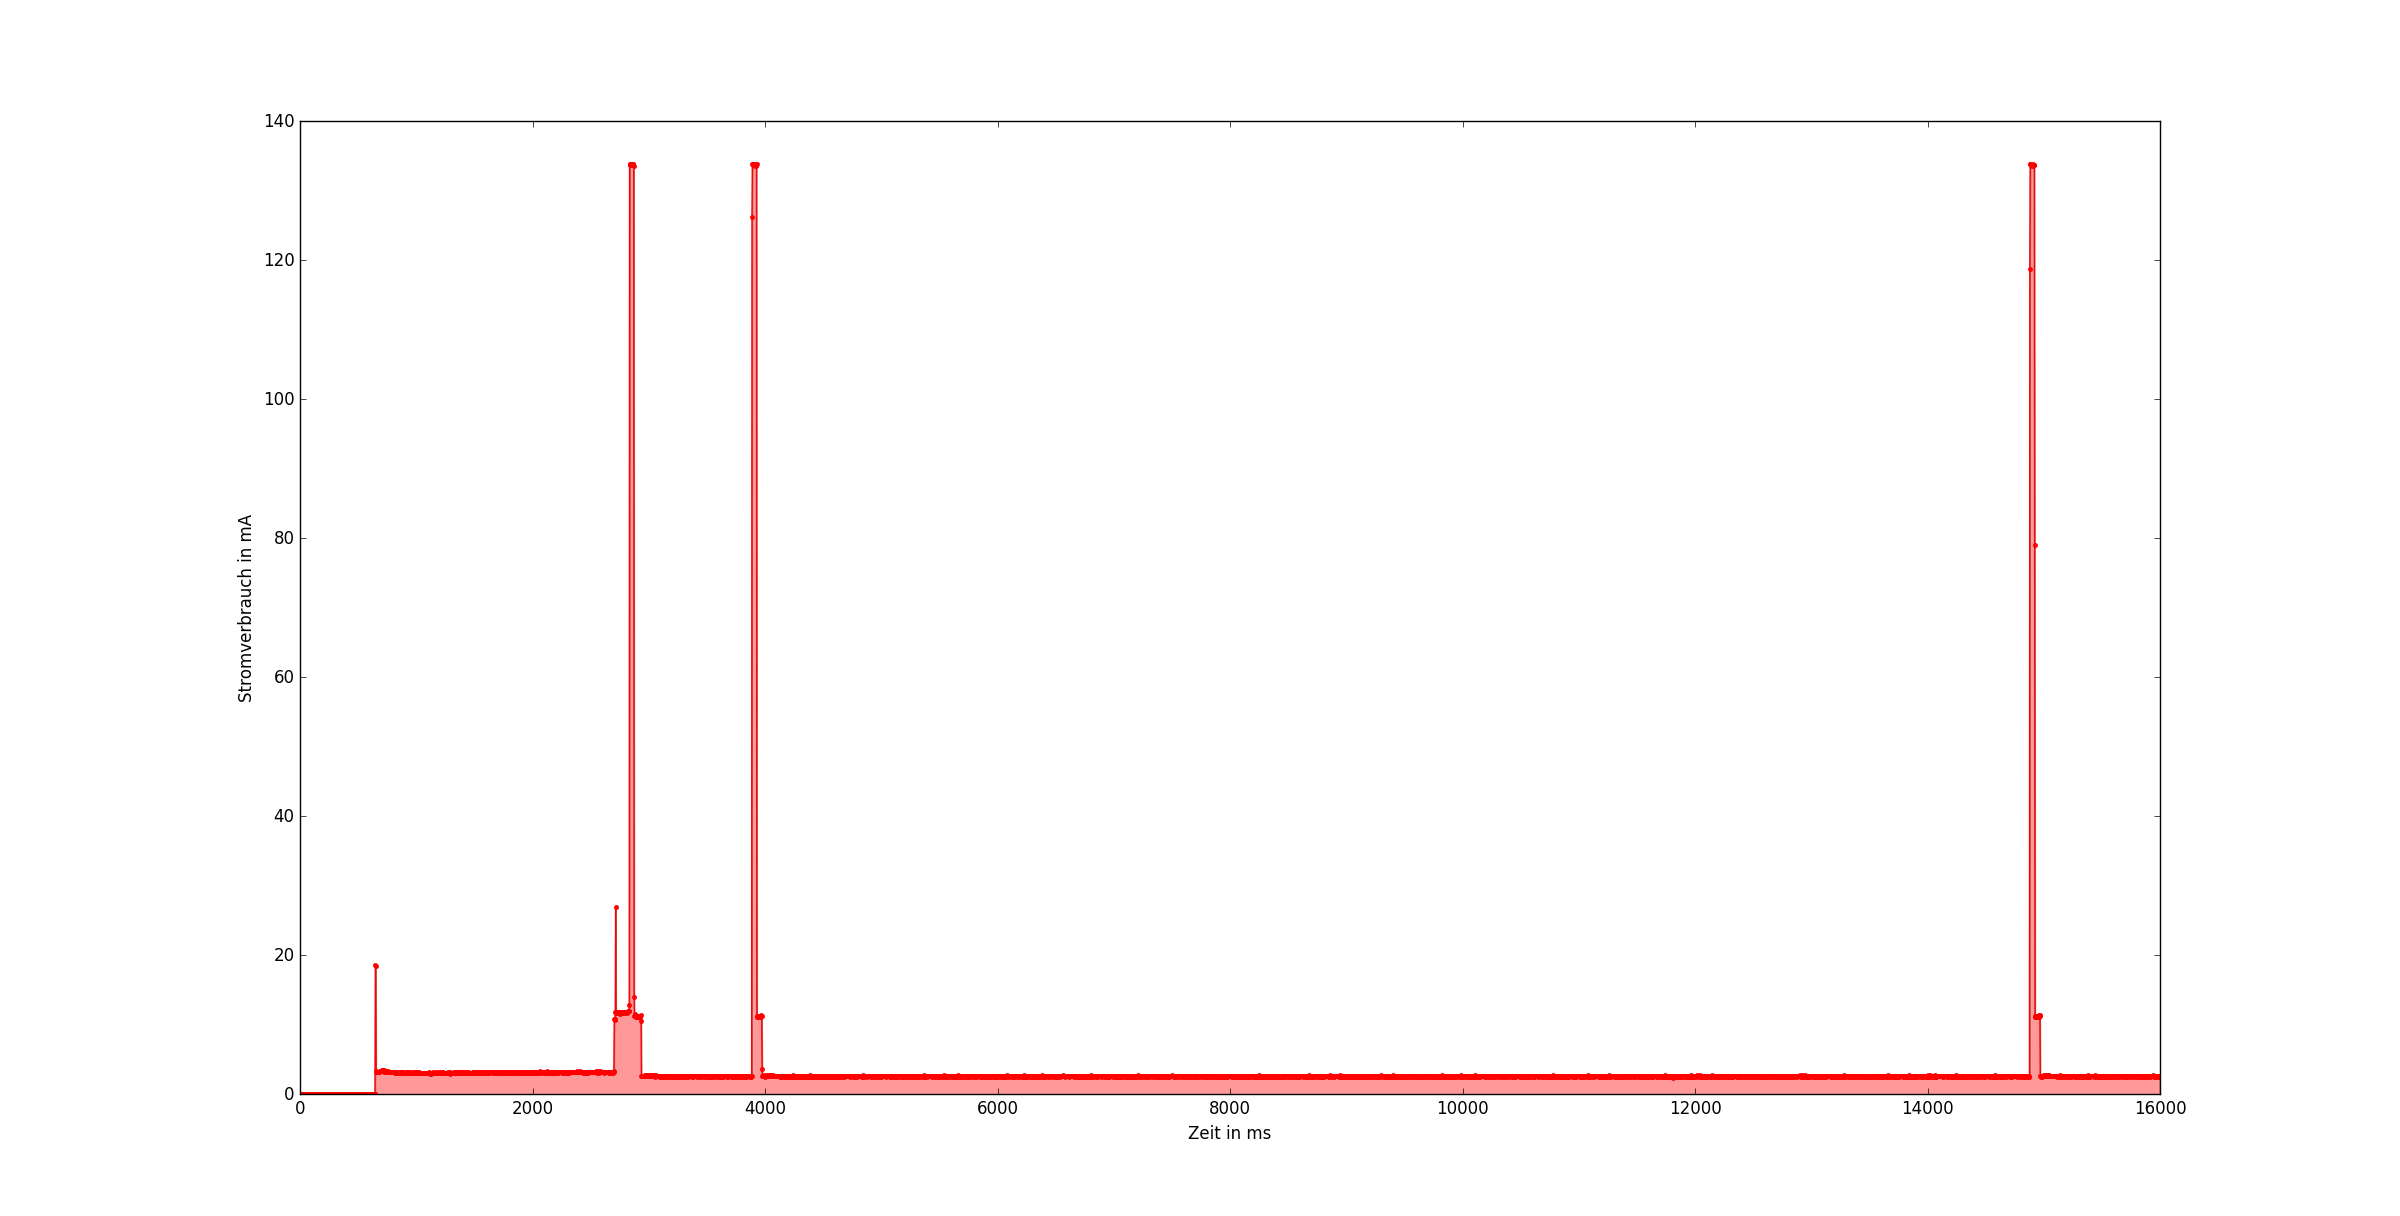
\includegraphics[width=\textwidth]{plots/lora23.png}
  \caption{Lastkurve einer Implementierung mit LoRa.}
  \label{fig:lora23}
\end{figure}

Die Abbildung \ref{fig:lora235send} zeigt die Sendeverbäuche für eine Sendeleistung von 23dBm in Rot und für 5dBm in Grün.
Gut zu erkennen ist hier auch, dass ein Sendevorgang bei LoRa deutlich länger als bei Bluetooth Low Energy dauert, obwohl vergleichbar viele Bits übertragen werden.

\begin{figure}[h!]
  \centering
	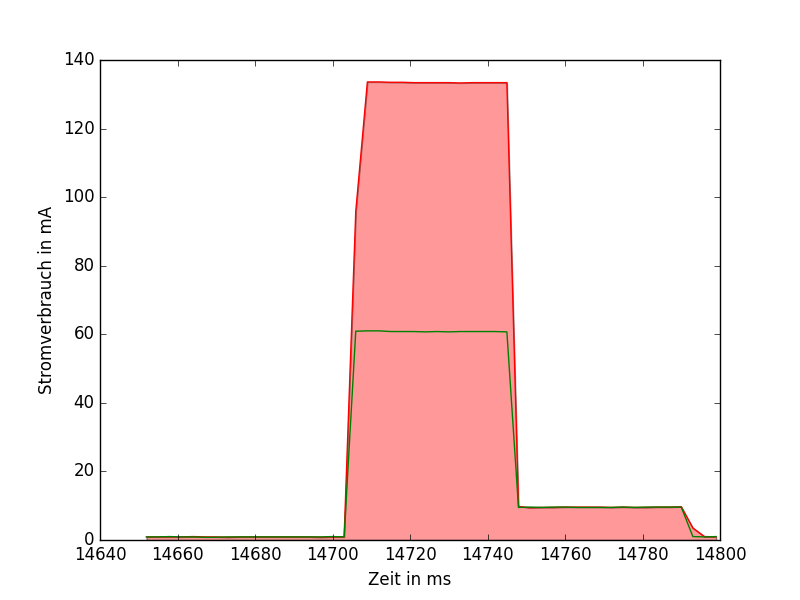
\includegraphics[width=\textwidth]{plots/lora235send.png}
  \caption{Lastkurve eines Ortungsvorgangs mit LoRa.}
  \label{fig:lora235send}
\end{figure}

Die Ergebnisse der Messungen sind in Tabelle \ref{table:lora235ina} gelistet.\\
Für den LoRa Feather liegt der Ruheverbrauch deutlich niedriger, da jedoch die selben Schaltungen für Akku-Ladung und Spannungsregelung zum Einsatz kommen scheint der CP2104, welcher zum Programmieren des ESP8266 beziehungsweise nRF52 dient, mindestens 4,5 Milliamper zu verbrauchen.

\begin{table}[h!]
	\centering
	\caption{Energieverbrauch mobiler Einheiten mit LoRa}
	\label{table:lora235ina}
	\begin{tabular}{p{3.5cm}|p{5cm}|p{2.5cm}|p{2.5cm}}
		Hardware & Programm & $\varnothing$ Verbrauch in mA & Laufzeit in Stunden\\
		\hline
		LoRa Feather & LoRa mit 23dBm Sendeleistung & 3,16 & 443\\
		LoRa Feather & LoRa mit 5dBm Sendeleistung & 2,88 & 486,1\\
	\end{tabular}
\end{table}

\section{Reichweite von Bluetooth}
Der Versuch mit Bluetooth wurde an der selben Stelle wie der mit WLAN durchgeführt, siehe dazu Abschitt \ref{ch:phase1:sec:rangewlan}.
Es wurde allerdings ein Raspberry Pi Zero W als Basisstation verwendet, dieser wurde auf dem LN-862 platziert, auf Abbildung \ref{fig:applacement} ist sein rotes Gehäuse zu erkennen.

\subsection{Methodik}
Die Reichweite wurde erneut in zwei Richtungen geprüft. 
Zum einen in Richtung der fertig gebohrten Tunnels mit wenigen Hindernissen, zum anderen in Richtung des Vortriebs durch mehrere Stahlhindernisse.
Um die Abschirmung durch ein Gehäuse zu simulieren wurde eine stabile Plastikbox verwendet, leider konnte diese nicht vollends geschlossen werden.\\
Für die Messung wurde der Körper zwischen mobile Einheit und Basisstation gebracht und eine mobile Einheit wurde dann als "außer Reichweite" angesehen, wenn versendete Pakete der mobilen Einheit nicht mehr bei der Basisstation ankamen.
Durch das Entfernen des körperlichen Hindernisses war es möglich wieder eine Verbindung herzustellen.\\
Die bestimmten Reichweiten werden in zwei Meter Schritten angegeben, da sie mit Hilfe der zwei Meter breiten Tübbing Elemente bestimmt wurden.

\subsection{Ergebnisse}
Tabelle \ref{table:rangeblue} zeigt die Ergebnisse für den nRF52.
Für diesen sind keine Ergebnisse mit geschlossenem Gehäuse aufgeführt, denn das Gehäuse ließ sich für diesen Prototyp nicht schließen.
Das lose Auflegen des Deckels führte zu keiner Veränderung bei der Reichweite.

\begin{table}[h]
	\centering
	\caption{Sendereichweite Bluetooth-basierter mobiler Einheiten}
	\label{table:rangeblue}
	\begin{tabular}{p{3.5cm}|p{3cm}|p{3.5cm}|p{3cm}}
		Verwendetes Modul & Aufbau & Strecke & Maximale Sendereichweite \\
		\hline
		nRF52 & Offen & Wenige Hindernisse & 32m \\
		nRF52 & In Gehäuse & Wenige Hindernisse & 32m \\
		nRF52 & Offen & Viele Hindernisse & 14m \\
		nRF52 & In Gehäuse & Viele Hindernisse & 14m \\
	\end{tabular}
\end{table}

\subsection{Bewertung}
Auch die mobile Einheit auf Bluetooth Basis hat eine höhere Reichweite als zunächst angenommen. 
Dennoch lohnt sich eine Anpassung des Sendeintervalls für die Lösung nicht, da der Großteil des Verbrauchs der mobilen Einheit passiv über die angrenzenden Komponenten wie Spannungswandler und Lithium-Akku-Ladeschaltkreis erfolgt.






\section{Reichweite von LoRa}
Die Versuche mit LoRa wurden an einer anderen Tunnelbaustelle durchgeführt.
An der Tunnelbohrstelle Ulm wird mit Sprengungen vorgetrieben.
Nach der Sprengung wird der Tunnel mit Spritzbeton ausgekleidet und danach wird in drei Schritten geschalt. 
Im ersten Schritt wird ein Filz und eine Folie gegen das Eindringen von Wasser eingebracht, danach folgt die Bewehrung und abschließend wird die Bewehrung einbetoniert.
Für jeden Schritt wird ein stählerner Schalungswagen verwendet, folglich sind drei stählerne Hindernisse im Tunnel, die Signale absorbieren.
Abbildung \ref{fig:schalungswagen} zeigt einen der Schalungswagen, der als Hindernis gedient hat.

\begin{figure}[h]
  \centering
	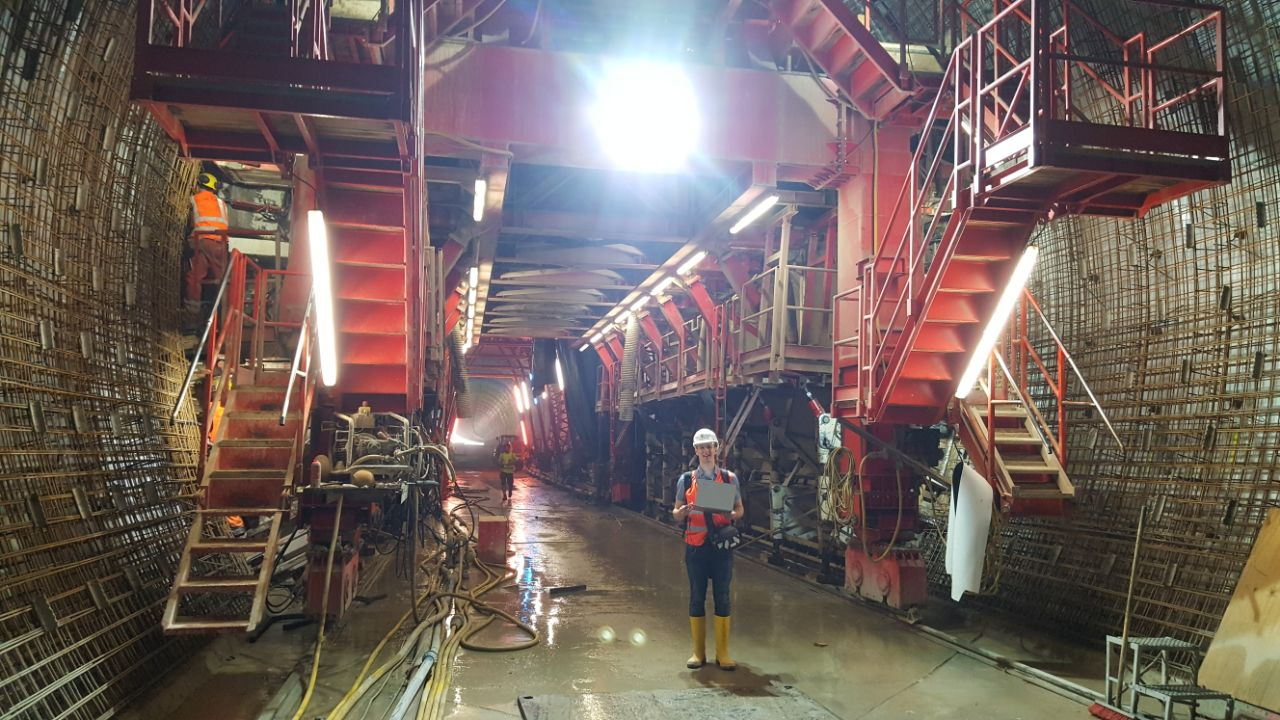
\includegraphics[width=\textwidth]{images/schalungswagen.jpg}
  \caption{Schalungswagen für das Betonieren im Tunnel Ulm.}
  \label{fig:schalungswagen}
\end{figure}

\subsection{Methodik} 
Die Reichweite wurde für zwei Situationen bestimmt.
Zum einen durch einen Schalungswagen und dann durch den freien Tunnel, zum anderen durch alle drei Schalungswagen für eine Situation mit maximaler Abschirmung durch die Hindernisse.
Die mobile Einheit wurde jeweils direkt an der Bewehrung platziert und es wurde auf der selben Seite gelaufen, damit die Abschirmung durch die Schalungswagen maximal ist.
Danach wurde die Basisstation immer weiter entfernt, bis keine Pakete der mobilen Einheit mehr empfangen werden konnten.
Abbildung \ref{fig:lorabasis} zeigt die Platzierung der mobilen Einheit an der Bewehrung.
Erneut konnte die Plastikbox aufgrund des Versuchsaufbaus nicht geschlossen werden.
Die mobile Einheit wurde als "{}außer Reichweite"{} angesehen, wenn versendete Pakete der mobilen Einheit nicht mehr bei der Basisstation ankamen.
Durch das Entfernen des körperlichen Hindernisses war es möglich wieder eine Verbindung herzustellen.
Es wurde sowohl mit einer Sendeleistung von 5dBm für einen geringen Sendeverbrauch als auch mit 23dBm Sendeleistung für maximale Reichweite gemessen.
Die Messungen werden in 12,5 Meter Abständen angegeben, da in diesem Tunnel die Länge eines Schalungselements 12,5 Meter beträgt.
Es werden, wie in Abschnitt \ref{ch:hardwarechanges:sec:rfm95} besprochen, zwei unterscheidliche Typen von Antennen verwendet. 
Während die Basisstation eine feste Antenne aufweist, verwendet die mobile Einheit eine Kabelantenne entsprechend der halben Wellenlänge. 

\begin{figure}[h]
  \centering
	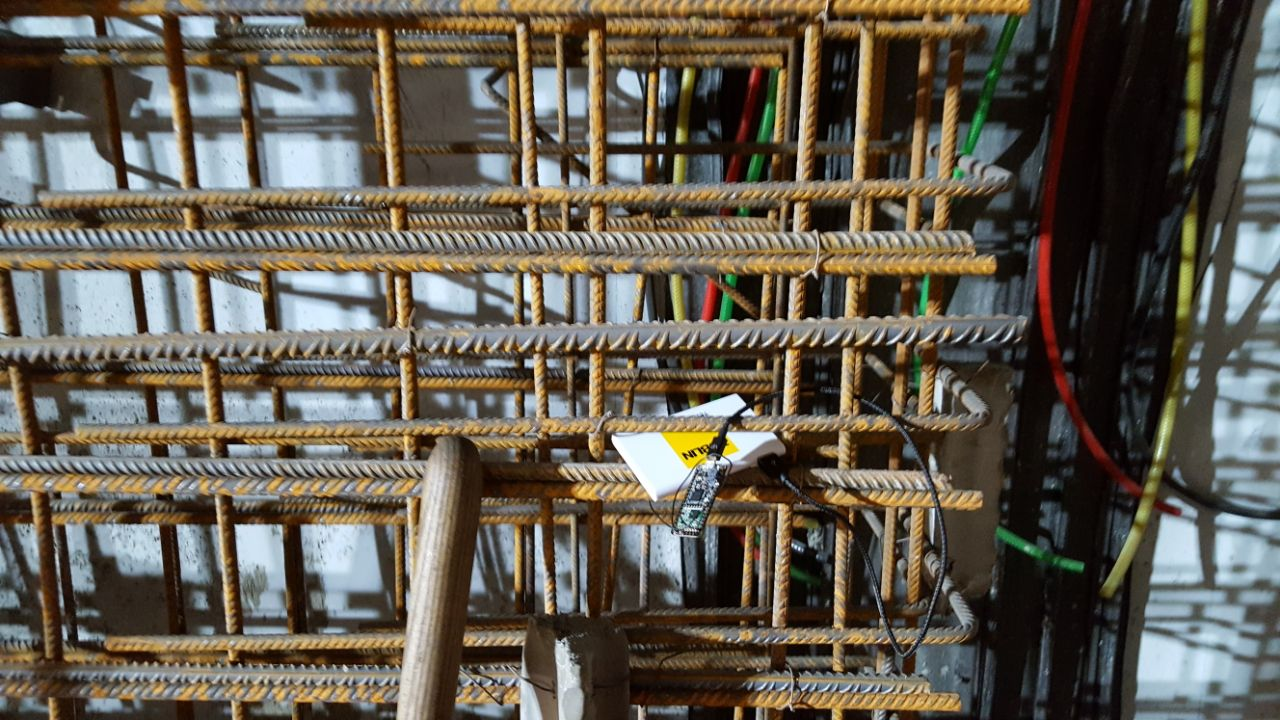
\includegraphics[width=\textwidth]{images/lorabasis.jpg}
  \caption{Platzierung der mobilen Einheit an der Bewehrung des Tunnels.}
  \label{fig:lorabasis}
\end{figure}

\subsection{Ergebnisse}
Tabelle \ref{table:rangelora} zeigt die Ergebnisse für das RFM95.
Da das lose Auflegen des Deckels der Plastikbox zu keiner Veränderung bei der Reichweite führte gibt die Tabelle nur Werte für den offenen Aufbau an. 
Der Test mit 23dBm Sendeleistung durch alle drei Schalungswagen musste nach 350 Metern abgebrochen werden, weil ein weiterkommen nicht möglich war.
Da jedoch für diese Sendeleistung bereits nach circa 250 Metern die Varianz des RSSI den Zusammenhang zwischen Distanz und RSSI überwiegt, kann die tatsächliche Reichweite dieser Sendeleistung nicht ausgenutzt werden.
Für eine sichere Erkennung des 250-Meter-Abschnitts müsste daher alle 500 Meter eine Basisstation aufgestellt werden.

\begin{table}[h]
	\centering
	\caption{Sendereichweite LoRa-basierter mobiler Einheiten}
	\label{table:rangelora}
	\begin{tabular}{p{2.2cm}|p{1.5cm}|p{2.5cm}|p{3.5cm}|p{3cm}}
		Verwendetes Modul & Aufbau & Sendeleistung & Strecke & Maximale Sendereichweite \\
		\hline
		RFM95 & Offen & 5dBm & Wenige Hindernisse & 250m \\
		RFM95 & Offen & 5dBm & Viele Hindernisse & 100m \\
		\hline
		RFM95 & Offen & 23dBm & Wenige Hindernisse & 1250m \\
		RFM95 & Offen & 23dBm & Viele Hindernisse & >350m \\
	\end{tabular}
\end{table}

\subsection{Bewertung}
LoRa entfaltet im Tunnel eine sehr hohe Reichweite und es kann eine lückenlose Überwachung von Personen durchgeführt werden.
Voll nutzen lässt sich diese jedoch nicht, da die Varianz des RSSI den Zusammenhang zwischen Distanz und RSSI schon nach circa 250 Metern überwiegt. 
Hingegen führt eine starke Reduktion der Sendeleistung zu einer mangelden Penetration von Hindernissen.
Daher sollte ein Kompromiss der Sendeleistung geschlossen werden. 
Eine Sendeleistung von 10dBm sollte eine ausreichende Reichweite im Szenario mit vielen Hindernissen bieten.
Alternativ kann die mobile Einheit auch ein Send-Receive Schema umsetzen und von der Basisstation eine dynamisch angepasste Sendeleistung empfangen, die sich nach der Menge der Hindernisse richtet.

